%*************************************************

\documentclass[a4paper,10pt]{article}
\usepackage[brazil]{babel}
\usepackage[utf8]{inputenc}
%\usepackage[latin1]{inputenc}
\usepackage{amsthm,amsfonts,amsmath,amssymb}
%img
\usepackage{graphicx}
\usepackage{subfig}
%fim
\usepackage{makeidx}
\usepackage{enumerate}
\usepackage{hyperref}
\hypersetup{
  colorlinks,
  linkcolor=blue,
  filecolor=blue,
  urlcolor=blue,
  citecolor=blue 
}
%titulo
\title{Servidor Concorrente TCP}
\author{Leandro Kümmel Tria Mendes RA033910 \\ Fernando Teixeira RA??????}
\makeindex
%inicio
\begin{document}
\maketitle
\tableofcontents
\listoffigures
\listoftables
\section{Introdução}
O objetivo desse projeto é implementar um sistema cliente/servidor
concorrente, com operações para o gerenciamento de livros em uma livraria.
Na comunicação entre cliente e servidor utilizou-se o protocolo TCP\footnote{
Mais informações sobre TCP \url{http://www.linktionary.com/t/tcp.html} }, da camada de transporte, e a partir da execução de testes podemos avaliar alguns aspectos
desse protocolo e posteriormente compará-lo com outro(s).
\section{Desenvolvimento}
Linux foi o sistema operacional utilizado para o desenvolvimento (distribuição
2.6.43.8-1.fc15.i686). Igualmente, para os testes utilizou-se duas máquinas com linux, porém com distribuições diferentes.
\subsection{Protocolo TCP - Transmission Control Protocol}
O protocolo TCP foi escrito de modo a garantir que os dados enviados (pelo
servido) e recebidos (pelo cliente) de forma correta, na sequência 
adequada e sem erros, pela rede.
\\As características fundamentais do TCP são:
\begin{itemize}
\item \emph{Orientado à conexão}: necessidade de uma conexão.
\item \emph{Ponto a ponto}: conexão é estabelecida entre dois pontos.
\item \emph{Confiabilidade}: Permite a recuperação de arquivos perdidos, elimina 
arquivos duplicados, recupera dados corrompidos, entrega na ordem do envio e 
pode recuperar o \"link\" entre cliente e servidor, caso esse, por algum motivo,
seja perdido.
\item \emph{Full duplex}: Possível transferência simultânea, entre cliente e 
servidor
\item \emph{Handshake}: Mecanismo de estabelecimento e finalização de conexão.
O TCP garante que, no final da conexão, \textbf{todos} os pacotes sejam entregues
/recebidos
\item \emph{Entrega ordenada}: A aplicação entrega ao TCP bloco de dados de 
tamanho variável. Esse protocolo divide estes dados em segmentos de tamanho 
especificado (valor MTU). Sabe-se que camadas inferiores a de transporte podem 
fazer com que os pacotes não cheguem na ordem em que foram enviados. Porém, o TCP
garante a reconstrução dos segmentos no cliente (TCP utiliza um número de 
sequência)
\item \emph{Controle de fluxo}: O protocolo em estudo utiliza-se de um campos 
denominado janela para controlar o fluxo
\end{itemize}
\subsection{Implementação}
O projeto conta com cinco diretórios, cada um com seu Makefile (exceto relatorio e estat), arquivos
principal (main.c e main.h) e um README.md\footnote{Leia esse arquivo antes de
executar o sistema} para instruções adicionais. Há também um Makefile, o qual 
compi
\\Os diretório são:
\begin{enumerate}[I.]
\label{sec:dirs}
\item \label{itm:common} \emph{common}: Contém arquivos de uso comum, tanto pelo servidor quanto 
pelo cliente, inclusive o arquivo que calcula a média dos testes executados.
\item \label{itm:server} \emph{server}: Contém os arquivos que preparam uma porta para esperar
conexões e manipulam o sistema de livraria.
\item \label{itm:client} \emph{client}: Funções que provêm conexão com um servidor, envio das opções
escolhidas pelo cliente e interface para as respostas do sistema de livraria
(servidor).
\item \label{itm:estat} \emph{estat}: Medidas de tempo efetuadas pelo teste.
\item \label{itm:relatorio} \emph{relatorio}
\end{enumerate}
\subsubsection{Manipulação de dados}
Todas as estruturas utilizadas para leitura/escrita dos livros são dinâmicas. \\Arquivos presentes no diretório \emph{common}[\ref{itm:common}]:
\begin{enumerate}[I.]
\item \emph{error.c error.h}: Gerencia erros que eventualmente podem ocorrer.
\item \emph{common.c common.h}: Funções de uso comum.
\item \label{itm:avl} \emph{avl.c avl.h}: Gerencia a estrutura básica da livraria, utiliza-se 
árvore AVL\footnote{ \url{http://pages.cs.wisc.edu/~ealexand/cs367/NOTES/AVL-Trees/index.html} }, pois a busca, inserção/atualização têm complexidade \boxed{O(logN)} , sendo N
o número de elementos na árvore, no caso a quantidade de livros diferentes.
\item \emph{archives.c archives.h}: Manipula arquivos. Faz a leitura do arquivo
da livraria\footnote{Ver README.md para mais detalhes do arquivo da livraria}.
\item \emph{tcp.c tcp.h}: Contém apenas algumas constantes.
\item \emph{books.c books.h}: Gerencia a estrutura básica de um livro e seus autores.
\item \label{itm:tempo}\emph{tempo.c tempo.h}: Gerencia a estrutura de testes, lê e escreve em arquivos localizados no diretório \emph{estat}[\ref{itm:estat}].
\item \emph{livros/livros}: Arquivo contendo os livros\footnote{Ver README.md para mais detalhes do arquivo da livraria}.
\end{enumerate}
\subsubsection{Conexão Servidor/Cliente}
Compreende dois diretórios \emph{server}[\ref{itm:server}] e \emph{client}[\ref{itm:client}]
\\\textbf{Servidor}:
\begin{enumerate}[I.]
\item \emph{server.c server.h}: Apenas inicia o servidor dada um número de uma porta.
\item \label{itm:tcpserver} \emph{tcp\_server.c tcp\_server.h}: Gerencia tanto as conexões com os clientes quanto a comunicação, em outras palavras, o tcp\_server.c recebe um stream do tcp\_client.c[\ref{itm:tcpclient}] e envia uma resposta adequada ao mesmo.
\item \emph{login.c login.h}: Gerencia o login necessário para editar a quantidade de um livro.
\end{enumerate}
\textbf{Cliente}:
\begin{enumerate}[I.]
\item \emph{client.c client.h}: Apenas inicia a comunicação com um servidor dado o endereço IP e um número de uma porta.
\item \label{itm:tcpclient} \emph{tcp\_client.c tcp\_client.h}: Gerencia tanto 
a criação de uma conexão entre o cliente e servidor quanto a leitura, da entrada dada pelo usuário do sistema, e a comunicação entre hospedeiro e cliente.
\end{enumerate}
\subsection{Coleta e gerência de dados para testes}
Para realizar os testes implementou-se alguns arquivos adicionas[\ref{itm:tempo}]. Uma constante, denominada NUM\_TESTES\footnote{Nesse sistema consideramos NUM\_TESTES igual a 100} , contém o número de testes a serem realizados, ou seja, cada opção do \emph{menu}[\ref{itm:tcpserver}] é executada NUM\_TESTE vezes. Todos os dados são 
salvos no diretório \emph{estat}[\ref{itm:estat}].
\subsection{Vantagens da implementação}
O sistema de livraria é um sistema robusto e com baixa complexidade de tempo.
A escolha da estrutura de árvore avl[\ref{itm:avl}], possibilitou em boa 
performance em questão de tempo de processamento, uma vez que, essa estrutura
mostrou-se eficaz para o problema e tem possuí melhor complexidade de tempo com 
relação a outras estruturas, além de ser de a implementação e manuntenção serem
simples.
\\ Com relação as conexões e comunicações entre cliente/servidor, vale ressaltar que há uma troca de mensagens\footnote{Sabe-se que o TCP envia/recebe streams} inicial entre os dois, na qual o conteúdo do stream
é o número de bytes da maior mensagem possível a ser enviada pelo servidor.
\begin{figure}[!htb]
  \centering
  \subfloat[Fluxograma Servidor]{
  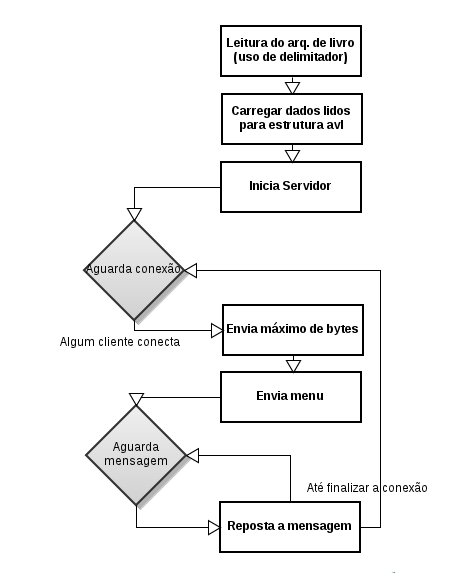
\includegraphics[width=150px,height=300px]{fluxo_servidor.png}
  \label{fluxoservidor}
  }
  \quad %espaco separador
   \subfloat[Fluxograma Cliente]{
     \label{fluxoserver}
     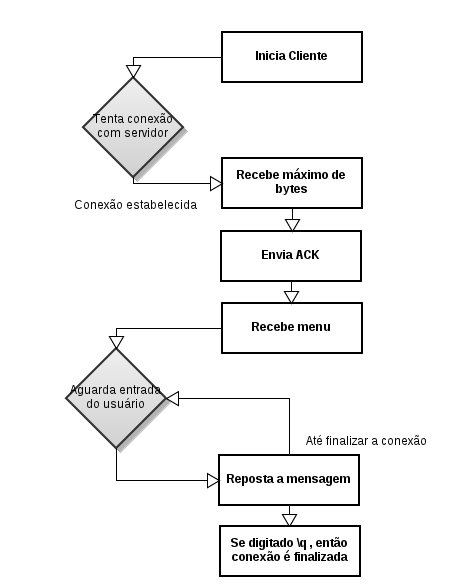
\includegraphics[width=150px,height=300px]{fluxo_cliente.png}
   }
   \caption{Fluxogramas}
   \label{figfluxos}
\end{figure}
\begin{figure}[!htb]
  \centering
  \label{fluxotempo}
  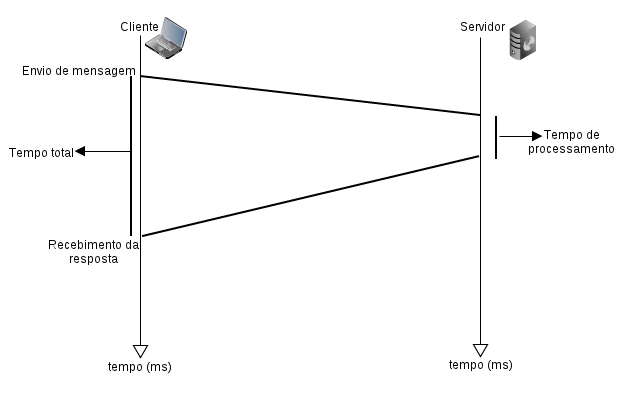
\includegraphics[scale=0.5]{fluxo_tempo.png}
  \caption{Definição do cálculo dos tempos}
\end{figure}
\end{document}
